\textbf{Пример}

Пусть $N=4$, $H=[2,4,3,5]$, $Q=2$, и $R=[2,3]$.

Проверяющий модуль (grader) делает вызов функции \texttt{minimum\_costs([2, 4, 3,
5], [0, 1], [2, 3])}.

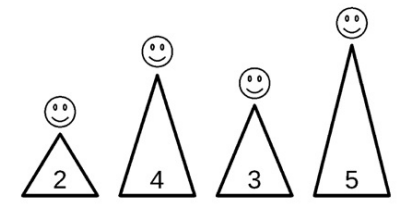
\includegraphics{1.png}


Для встречи с номером $j=0$ имеем $L_j=0$ и $R_j=2$, таким образом, в ней примут
участие жители гор с номерами $0$, $1$ и $2$. Если гора с номером $0$ выбрана в качестве
места встречи, то стоимость встречи с номером $0$ вычисляется следующим
образом:
\begin{itemize}
    \item Стоимость для участника, живущего на горе с номером $0$, равна $\max(H_0)=2$.
    \item Стоимость для участника, живущего на горе с номером $1$, равна $\max(H_0, H_1)=4$.
    \item Стоимость для участника, живущего на горе с номером $2$, равна $\max(H_0, H_1, H_2)=4$.
    \item Следовательно, стоимость встречи с номером $0$ равна $2 + 4 + 4 = 10$.

\end{itemize}
Невозможно организовать встречу с номером $0$ с меньшей стоимостью, поэтому
минимальная стоимость встречи $0$ равна $10$.

Для встречи с номером $j=1$ имеем $L_j = 1$ и $R_j=3$, таким образом, в ней примут
участие жители гор с номерами $1$, $2$ и $3$. Если гора с номером $2$ выбрана в качестве
места встречи, то стоимость встречи с номером $1$ вычисляется следующим
образом:
\begin{itemize}
    \item Стоимость для участника, живущего на горе с номером $1$, равна $\max(H_1, H_2)=4$.
\item Стоимость для участника, живущего на горе с номером $2$, равна $\max(H_2)=3$.
\item Стоимость для участника, живущего на горе с номером $3$, равна $\max(H_2, H_3)=5$.
\item Следовательно, стоимость встречи с номером $1$ равна $4 + 3 + 5 = 12$.

\end{itemize}


Невозможно организовать встречу с номером $1$ с меньшей стоимостью, поэтому
минимальная стоимость встречи $1$ равна $12$.

Файлы sample-01-in.txt и sample-01-out.txt в приложенном zip-архиве
соответствуют этому примеру. В архиве есть также другие примеры ввода и
вывода.
